\chapterimage{chapter_head_1.png}

\chapter{Informierte Suche}

\section{Einf\"uhrung und Motivation}
Im vorherigen Kapitel haben wir bereits einige Algorithmen zur uninformierten (\glqq blinden\grqq) Suche, wie die Breitensuche und Tiefensuche kennengelernt. Diese haben jedoch im Allgemeinen einen recht hohen Aufwand und garantieren teilweise nicht für das Finden einer Lösung (->Tiefensuche in unendlichen Bäumen). Daher haben wir ebenfalls zwei einfache informierte Suchalgorithmen kennengelernt, nämlich Hill-Climbing und Beam-Search. Jedoch bringen auch diese noch einige Schwierigkeiten mit sich.
Deshalb werden wir uns in diesem Kapitel tiefergehend mit informierter Suche beschäftigen.
Es soll vor allem darum gehen Algorithmen kennenzulernen, welche durch Einbeziehen von zusätzlichem heuristischen Wissen einen geringeren Aufwand zum Erreichen eines Ziels benötigen und gleichzeitig die Kosten einer Lösung mit einbeziehen.
Ebenfalls beschäftigen werden wir uns mit der Zulässigkeit und der Optimalität dieser Algorithmen.
Im Näheren werden wir Branch and Bound und Best-First-Search (Bestensuche) kennenlernen. Das bekannteste Verfahren aus dem Bereich Best-First-Search ist der Algorithmus A*, welcher in der folgenden Ausarbeitung besonders genau erläutert und an einigen Beispielen verdeutlicht wird.



\section{Problemstellung}

In diesem Kapitel geht es um das Lösen verschiedener Probleme mittels heuristischer Suche, welche durch heuristische Suche in entsprechenden Graphen modelliert wird.
Reale Beispiele solcher Probleme sind Routenberechnungsprobleme, Navigationsprobleme, das Travelling Salesman Problem und das Problem von Roboternavigation. Aber auch abstraktere Probleme, wie das 8-Puzzle und das 8-Damen-Problem, lassen sich durch entsprechende heuristische Suchen lösen.

Wir haben also einen Suchraum mit verschiedenen Zuständen des Problems gegeben. Diese entsprechen den Knoten des dazugehörigen Problemgraphen $G_{P}$=(V,E).
Die Kanten des Graphen entsprechen den Übergangsoperationen der Zustände.
Die Zielknoten entsprechen den Zielzuständen, und der Startknoten dem Startzustand.

Des Weiteren existiert eine Kostenfunktion für die Überführung der einzelnen Zustände. Dementsprechend gibt es eine Gewichtsfunktion $c:E\to \mathbb{N}$, welche jeder Kante des Problemgraphen feste Kosten zuordnet.

Die Aufgabe ist nun in diesem Problemgraphen einen Weg zu finden, und zwar von einem gegebenen Startzustand zu einem Zustand, welcher eine festgelegte Zielbedingung erfüllt.
Dieser Weg soll dabei möglichst geringe Kosten haben. Das heißt, man sucht bezüglich der gegebenen Kostenfunktion nach einer optimalen Lösung des Problems.

Einige Suchalgorithmen zur Lösung dieses Problems, welche in diesem Kapitel erörtert werden, nutzen eine heuristische Komponente.
Diese hat den Zweck, den Aufwand zum Finden dieser optimalen Lösung möglichst gering zu halten.




\section{Branch and Bound}

Die Idee, auf welcher Branch and Bound beruht, ist folgende. Hat man für seinen Problemgraphen einen Lösungspfad gegeben und möchte wissen, ob dies auch eine optimale Lösung ist, so genügt es, alle restlichen Pfade nur so weit zu betrachten, bis ihre Kosten größer werden als jene des bekannten Lösungspfades.
In der Umsetzung des Algorithmus sieht dies wie folgt aus.

\subsection{Intuitiver Algorithmus}

Startknoten $s$ wird in den Such-Baum $G_{S}$ eingefügt. Anbei wird der Wert $g(s)=0$ gespeichert, welcher die Kosten zum Erreichen dieses Knotens repräsentiert.
Nun wird folgende Schleife behandelt, und zwar so lange, bis es keinen unbehandelten Knoten mehr gibt.
Wähle aus den noch unbehandelten Blättern des Such-Baums $G_{S}$ denjenigen Knoten $n$ mit geringsten Kosten $g(n)$ vom Startknoten $s$ bis nach $n$. (Gibt es mehrere Knoten mit dem selben minimalen Wert, dann wähle von diesen zufällig einen aus.)
Ist $n$ ein Zielknoten, so terminiert die Suche erfolgreich und der Pfad vom Startknoten $s$ nach $n$ ist eine optimale Lösung.
Ansonsten erweitere den Such-Baum $G_{S}$ durch Anhängen aller möglichen Nachfolger an Knoten $n$. (Lasse dabei alle Knoten aus, welche bereits auf dem Pfad von $s$ nach $n$ vorkommen.) Berechne dann für jeden dieser Nachfolger $t$ die Pfadkosten bis nach $t$. Addiere dafür die Kosten der Kante von $n$ nach $t$ auf die Pfadkosten des Vaters $n$ auf: $g(t)=c({n,t})+g(n)$.

Veranschaulichen wir den Algorithmus nun an folgendem Beispiel. Gegeben sei ein Problemgraph mit eingezeichneter Kostenfunktion. S sei der Startknoten und G der Zielknoten. Der entstehende Such-Baum $G_{S}$ ist ebenfalls auf der kommenden Seite dargestellt.

\begin{figure}[h!]
	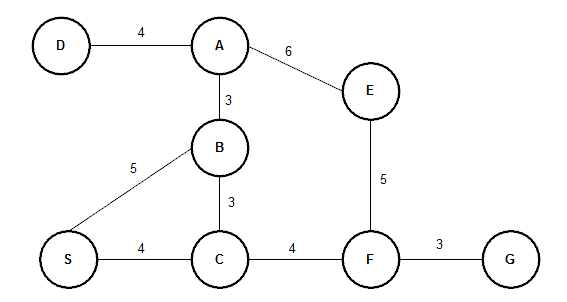
\includegraphics[scale=0.6]{chapters/informed_search/bab.png}
	\caption{Problemgraph}
	\label{fig:figure3}
\end{figure}

\begin{figure}[h!]
	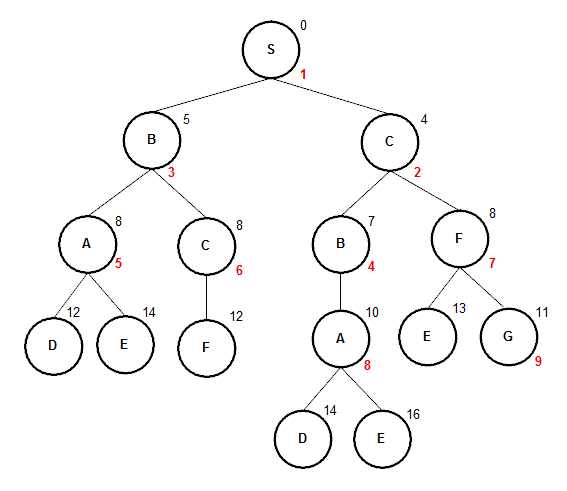
\includegraphics[scale=0.6]{chapters/informed_search/babsearch.png}
	\caption{Such-Baum $G_{S}$}
	\label{fig:figure4}
\end{figure}

Der gefundene optimale Pfad lautet hier (S,C,F,G).
Die roten Zahlen geben an, in welcher Reihenfolge die Knoten betrachtet werden. Die schwarzen Zahlen sind die berechneten Pfadkosten.

Nachdem wir diesen intuitiven Algorithmus verstanden haben, möchte ich noch eine Implementierung von Branch and Bound angeben, welche die Suche mittels einer Queue (Warteschlange) realisiert. In dieser werden zur Laufzeit des Algorithmus die bisher aufgebauten Pfade gespeichert und geordnet.

\subsection{Implementierung mittels Queue}

\begin{itemize}
	\item Initialisiere die Queue.
	\item Erzeuge einen Pfad, welcher nur aus dem Startknoten besteht, und schreibe ihn in die Queue.
	\item Solange der erste Pfad in der Queue nicht mit einem Zielknoten endet und die Queue nicht leer ist:
	\begin{itemize}
		\item Nehme den ersten Pfad aus der Queue. Ermittle den Endknoten dieses Pfades und erzeuge für jeden Nachbarn dieses Endknotens je einen neuen Pfad, indem dieser an den bisherigen Pfad angehangen wird.
		\item Entferne alle neuen Pfade, welche Schleifen enthalten.
		\item Füge die übrigen Pfade in die Queue ein.
		\item Sortiere die Queue aufsteigend nach den Pfadkosten.
	\end{itemize}
	\item Falls ein Zielknoten erreicht wurde, gib den Pfad als Lösung aus.
\end{itemize}

\section{Best-First Search} \label{BFS}

Best-First Search ist eine Klasse von informierten Such-Algorithmen, welche nach dem Prinzip arbeiten, dass sie stets denjenigen Knoten zuerst untersuchen, welcher für den Erfolg der Suche am \glqq vielversprechendsten\grqq\ erscheint. Die Wahl dieses \glqq vielversprechenden\grqq\ Knotens geschieht anhand einer gewissen Heuristik.
Der wohl bekannteste Algorithmus aus diesem Bereich ist A*, welcher auch als eine Erweiterung von Branch and Bound gesehen werden kann. An ihm wollen wir im Folgenden das Prinzip von Best-First Search verdeutlichen.

\subsection{A* Algorithmus}

Die verwendete Heuristik sei mit $f(n)$ bezeichnet und auf allen Knoten $n$ des Problemgraphen $G_{P}$ definiert. Somit ist $f$ auch für alle Knoten des später aufgebauten Such-Graphen $G_{S}$ definiert.

Die Idee des Algorithmus besteht darin, dass die Kosten eines optimalen Pfades durch Knoten $n$ als Summe der Kosten vom Start zu $n$ und der Kosten von $n$ zu einem Ziel dargestellt werden.
Dazu definieren wir folgende Funktionen:

\begin{description}
	\item[$g^{*}(n)$]{Kosten eines optimalen Pfades vom Start zu $n$}
	\item[$h^{*}(n)$]{Kosten eines optimalen Pfades von $n$ zu einem Knoten, welcher die Endbedingung erfüllt}
	\item[$f^{*}(n)$]{Kosten eines optimalen Pfades vom Start über $n$ zu einem Knoten, welcher die Endbedingung erfüllt}
\end{description}
Also gilt: \[f^{*}(n)=g^{*}(n)+h^{*}(n)\]


Da zum Zeitpunkt der Suche für gewöhnlich aber kein Wissen über die tatsächlichen Kosten eines solchen optimalen Pfades vorliegt, ist es an diesem Punkt nötig, eine Schätzung für $g^{*}(n)$ und $h^{*}(n)$ einzuführen.
Wir definieren:

\begin{description}
	\item[$g(n)$]{Kosten des günstigsten bisher gefundenen Pfades vom Start zu $n$}
	\item[$ h(n)$]{geschätzte Kosten von $n$ zu einem Knoten, welcher die Endbedingung erfüllt}
	\item[$ f(n)$]{geschätzte Kosten eines optimalen Pfades vom Start über $n$ zu einem Knoten, welcher die Endbedingung erfüllt

		-> resultierende Heuristikfunktion}
\end{description}
Auch hier gilt: \[f(n)=g(n)+h(n)\]

Die Funktion $g$ lässt sich dabei leicht mittels des bisher aufgebauten Such-Baumes $G_{S}$ bestimmen, indem die einzelnen Kantengewichte aufsummiert werden.
Es ist zu bemerken, dass durch diese Art der Pfadbewertung der heuristische Wert $g$ niemals die tatsächlichen Kosten $g^{*}$ unterschreitet.
Es gilt also $g(n) \geq g^{*}(n)$ für alle $n \in G_{P}$.
(Denkbar wären auch andere Funktionen, aus denen sich die Bewertungen eines Pfades berechnen. Beispielsweise könnte statt der Summe der Kantengewichte auch das Produkt, Maximum oder der Median herangezogen werden. Welche Auswirkungen dies mit sich bringt, wird an dieser Stelle offen gelassen. Der interessierte Leser kann eine genauere Behandlung dieser Fälle in \cite{Dechter:1985:GBS:3828.3830} nachlesen.)

\subsection{Beispiel}

Wir wollen nun den $\text{A}^*$ Algorithmus an einem Beispiel anwenden.
Sei dazu der Graph $G$ und die Heuristik $h$ durch
\fbox{
\begin{tikzpicture}[auto, node distance=2cm, every loop/.style={},
                    thick,main node/.style={circle,draw,font=\sffamily\Large\bfseries}]

  \node[main node, label={\color{red}\small 9}] (1) at (1, 3) {1};
  \node[main node, label={\color{red}\small 6}] (2) at (4, 3) {2};
  \node[main node, label={\color{red}\small 7}] (3) at (3, 4) {3};
  \node[main node, label={\color{red}\small 5}] (4) at (5, 4) {4};
  \node[main node, label=left:{\color{red}\small 5}] (5) at (5, 1) {5};
  \node[main node, label={\color{red}\small 1}] (6) at (9, 3) {6};
  \node[main node, label={\color{red}\small 2}] (7) at (8, 4) {7};
  \node[main node, label=left:{\color{red}\small 2}] (8) at (8, 1) {8};
  \node[main node, label={\color{red}\small 8}] (9) at (2, 1) {S};
  \node[main node, label={\color{red}\small 0}] (10) at (10, 2) {Z};

  \path[every node/.style={font=\sffamily\small}]
  (9) edge node [sloped, below] {2.5} (1)
  (1) edge node [sloped] {3} (2)
  (2) edge node [sloped, above] {4.5} (7)
  (7) edge node [left, yshift=0.5cm] {3} (8)
  (8) edge node [sloped, above] {2.5} (10)
  (9) edge node [sloped] {3.5} (3)
  (3) edge node [sloped] {2} (4)
  (4) edge node [right] {3} (5)
  (5) edge node [sloped] {4.5} (6)
  (6) edge node [sloped, above] {1.5} (10)
  (4) edge node [sloped, above] {1.5} (2);

\end{tikzpicture}}\vspace{5pt}\\
gegeben. Wir wollen einen Weg von $S$ nach $Z$ suchen. Man erhält Folgendes:
(hierbei ist eine Zahl im Knoten rot, falls er in der Extended-List
ist, grün wenn er gerade expandiert wird und gelb falls er auf der Open-List
ist):\vspace{5pt}\\
\fbox{
\begin{tikzpicture}[auto, node distance=2cm, every loop/.style={},
                    thick,main node/.style={circle,draw,font=\sffamily\Large\bfseries}]

  \node[main node, label={\color{red}\small 9}] (1) at (1, 3) {1};
  \node[main node, label={\color{red}\small 6}] (2) at (4, 3) {2};
  \node[main node, label={\color{red}\small 7}] (3) at (3, 4) {3};
  \node[main node, label={\color{red}\small 5}] (4) at (5, 4) {4};
  \node[main node, label=left:{\color{red}\small 5}] (5) at (5, 1) {5};
  \node[main node, label={\color{red}\small 1}] (6) at (9, 3) {6};
  \node[main node, label={\color{red}\small 2}] (7) at (8, 4) {7};
  \node[main node, label=left:{\color{red}\small 2}] (8) at (8, 1) {8};
  \node[main node, color=green, label={\color{red}\small 8}] (9) at (2, 1) {S};
  \node[main node, label={\color{red}\small 0}] (10) at (10, 2) {Z};

  \path[every node/.style={font=\sffamily\small}]
  (9) edge node [sloped, below] {2.5} (1)
  (1) edge node [sloped] {3} (2)
  (2) edge node [sloped, above] {4.5} (7)
  (7) edge node [left, yshift=0.5cm] {3} (8)
  (8) edge node [sloped, above] {2.5} (10)
  (9) edge node [sloped] {3.5} (3)
  (3) edge node [sloped] {2} (4)
  (4) edge node [right] {3} (5)
  (5) edge node [sloped] {4.5} (6)
  (6) edge node [sloped, above] {1.5} (10)
  (4) edge node [sloped, above] {1.5} (2);

\end{tikzpicture}}
\hfill
\fbox{\begin{minipage}[b][4.27cm][t]{0.34\textwidth}
    \begin{tabular}{|l|r|}
      Queue & Prio\\
      (S) & 8\\
      \phantom{(S, 3, 4, 5, 6, Z)} & \phantom{14.5}
    \end{tabular}
\end{minipage}}\vspace{5pt}\\
\fbox{
\begin{tikzpicture}[auto, node distance=2cm, every loop/.style={},
                    thick,main node/.style={circle,draw,font=\sffamily\Large\bfseries}]

  \node[main node, color=yellow, label={\color{red}\small 9}] (1) at (1, 3) {1};
  \node[main node, label={\color{red}\small 6}] (2) at (4, 3) {2};
  \node[main node, color=green, label={\color{red}\small 7}] (3) at (3, 4) {3};
  \node[main node, label={\color{red}\small 5}] (4) at (5, 4) {4};
  \node[main node, label=left:{\color{red}\small 5}] (5) at (5, 1) {5};
  \node[main node, label={\color{red}\small 1}] (6) at (9, 3) {6};
  \node[main node, label={\color{red}\small 2}] (7) at (8, 4) {7};
  \node[main node, label=left:{\color{red}\small 2}] (8) at (8, 1) {8};
  \node[main node, color=red, label={\color{red}\small 8}] (9) at (2, 1) {S};
  \node[main node, label={\color{red}\small 0}] (10) at (10, 2) {Z};

  \path[every node/.style={font=\sffamily\small}]
  (9) edge node [sloped, below] {2.5} (1)
  (1) edge node [sloped] {3} (2)
  (2) edge node [sloped, above] {4.5} (7)
  (7) edge node [left, yshift=0.5cm] {3} (8)
  (8) edge node [sloped, above] {2.5} (10)
  (9) edge node [sloped] {3.5} (3)
  (3) edge node [sloped] {2} (4)
  (4) edge node [right] {3} (5)
  (5) edge node [sloped] {4.5} (6)
  (6) edge node [sloped, above] {1.5} (10)
  (4) edge node [sloped, above] {1.5} (2);

\end{tikzpicture}}\hfill
\fbox{\begin{minipage}[b][4.27cm][t]{0.34\textwidth}
    \begin{tabular}{|l|r|}
      Queue & Prio\\
      (S, 3) & 10\\
      (S, 1) & 11.5\\
      \phantom{(S, 3, 4, 5, 6, Z)} & \phantom{14.5}
    \end{tabular}
\end{minipage}}
\vspace{5pt}\\
\fbox{
\begin{tikzpicture}[auto, node distance=2cm, every loop/.style={},
                    thick,main node/.style={circle,draw,font=\sffamily\Large\bfseries}]

  \node[main node, color=yellow, label={\color{red}\small 9}] (1) at (1, 3) {1};
  \node[main node, label={\color{red}\small 6}] (2) at (4, 3) {2};
  \node[main node, color=red, label={\color{red}\small 7}] (3) at (3, 4) {3};
  \node[main node, color=green, label={\color{red}\small 5}] (4) at (5, 4) {4};
  \node[main node, label=left:{\color{red}\small 5}] (5) at (5, 1) {5};
  \node[main node, label={\color{red}\small 1}] (6) at (9, 3) {6};
  \node[main node, label={\color{red}\small 2}] (7) at (8, 4) {7};
  \node[main node, label=left:{\color{red}\small 2}] (8) at (8, 1) {8};
  \node[main node, color=red, label={\color{red}\small 8}] (9) at (2, 1) {S};
  \node[main node, label={\color{red}\small 0}] (10) at (10, 2) {Z};

  \path[every node/.style={font=\sffamily\small}]
  (9) edge node [sloped, below] {2.5} (1)
  (1) edge node [sloped] {3} (2)
  (2) edge node [sloped, above] {4.5} (7)
  (7) edge node [left, yshift=0.5cm] {3} (8)
  (8) edge node [sloped, above] {2.5} (10)
  (9) edge node [sloped] {3.5} (3)
  (3) edge node [sloped] {2} (4)
  (4) edge node [right] {3} (5)
  (5) edge node [sloped] {4.5} (6)
  (6) edge node [sloped, above] {1.5} (10)
  (4) edge node [sloped, above] {1.5} (2);

\end{tikzpicture}}\hfill
\fbox{\begin{minipage}[b][4.27cm][t]{0.34\textwidth}
    \begin{tabular}{|l|r|}
      Queue & Prio\\
      (S, 3, 4) & 10\\
      (S, 1) & 11.5\\
      \phantom{(S, 3, 4, 5, 6, Z)} & \phantom{14.5}
    \end{tabular}
\end{minipage}}\vspace{5pt}\\
\fbox{
\begin{tikzpicture}[auto, node distance=2cm, every loop/.style={},
                    thick,main node/.style={circle,draw,font=\sffamily\Large\bfseries}]

  \node[main node, color=green, label={\color{red}\small 9}] (1) at (1, 3) {1};
  \node[main node, color=yellow, label={\color{red}\small 6}] (2) at (4, 3) {2};
  \node[main node, color=red, label={\color{red}\small 7}] (3) at (3, 4) {3};
  \node[main node, color=red, label={\color{red}\small 5}] (4) at (5, 4) {4};
  \node[main node, color=yellow, label=left:{\color{red}\small 5}] (5) at (5, 1) {5};
  \node[main node, label={\color{red}\small 1}] (6) at (9, 3) {6};
  \node[main node, label={\color{red}\small 2}] (7) at (8, 4) {7};
  \node[main node, label=left:{\color{red}\small 2}] (8) at (8, 1) {8};
  \node[main node, color=red, label={\color{red}\small 8}] (9) at (2, 1) {S};
  \node[main node, label={\color{red}\small 0}] (10) at (10, 2) {Z};

  \path[every node/.style={font=\sffamily\small}]
  (9) edge node [sloped, below] {2.5} (1)
  (1) edge node [sloped] {3} (2)
  (2) edge node [sloped, above] {4.5} (7)
  (7) edge node [left, yshift=0.5cm] {3} (8)
  (8) edge node [sloped, above] {2.5} (10)
  (9) edge node [sloped] {3.5} (3)
  (3) edge node [sloped] {2} (4)
  (4) edge node [right] {3} (5)
  (5) edge node [sloped] {4.5} (6)
  (6) edge node [sloped, above] {1.5} (10)
  (4) edge node [sloped, above] {1.5} (2);

\end{tikzpicture}}\hfill
\fbox{\begin{minipage}[b][4.27cm][t]{0.34\textwidth}
    \begin{tabular}{|l|r|}
      Queue & Prio\\
      (S, 1) & 11.5\\
      (S, 3, 4, 2) & 13\\
      (S, 3, 4, 5) & 13.5\\
      \phantom{(S, 3, 4, 5, 6, Z)} & \phantom{14.5}
    \end{tabular}
\end{minipage}}\vspace{5pt}\\
\fbox{
\begin{tikzpicture}[auto, node distance=2cm, every loop/.style={},
                    thick,main node/.style={circle,draw,font=\sffamily\Large\bfseries}]

  \node[main node, color=red, label={\color{red}\small 9}] (1) at (1, 3) {1};
  \node[main node, color=green, label={\color{red}\small 6}] (2) at (4, 3) {2};
  \node[main node, color=red, label={\color{red}\small 7}] (3) at (3, 4) {3};
  \node[main node, color=red, label={\color{red}\small 5}] (4) at (5, 4) {4};
  \node[main node, color=yellow, label=left:{\color{red}\small 5}] (5) at (5, 1) {5};
  \node[main node, label={\color{red}\small 1}] (6) at (9, 3) {6};
  \node[main node, label={\color{red}\small 2}] (7) at (8, 4) {7};
  \node[main node, label=left:{\color{red}\small 2}] (8) at (8, 1) {8};
  \node[main node, color=red, label={\color{red}\small 8}] (9) at (2, 1) {S};
  \node[main node, label={\color{red}\small 0}] (10) at (10, 2) {Z};

  \path[every node/.style={font=\sffamily\small}]
  (9) edge node [sloped, below] {2.5} (1)
  (1) edge node [sloped] {3} (2)
  (2) edge node [sloped, above] {4.5} (7)
  (7) edge node [left, yshift=0.5cm] {3} (8)
  (8) edge node [sloped, above] {2.5} (10)
  (9) edge node [sloped] {3.5} (3)
  (3) edge node [sloped] {2} (4)
  (4) edge node [right] {3} (5)
  (5) edge node [sloped] {4.5} (6)
  (6) edge node [sloped, above] {1.5} (10)
  (4) edge node [sloped, above] {1.5} (2);

\end{tikzpicture}}\hfill
\fbox{\begin{minipage}[b][4.27cm][t]{0.34\textwidth}
    \begin{tabular}{|l|r|}
      Queue & Prio\\
      (S, 1, 2) & 11.5\\
      (S, 3, 4, 2) & 13\\
      (S, 3, 4, 5) & 13.5\\
      \phantom{(S, 3, 4, 5, 6, Z)} & \phantom{14.5}
    \end{tabular}
\end{minipage}}\vspace{5pt}\\
\fbox{
\begin{tikzpicture}[auto, node distance=2cm, every loop/.style={},
                    thick,main node/.style={circle,draw,font=\sffamily\Large\bfseries}]

  \node[main node, color=red, label={\color{red}\small 9}] (1) at (1, 3) {1};
  \node[main node, color=red, label={\color{red}\small 6}] (2) at (4, 3) {2};
  \node[main node, color=red, label={\color{red}\small 7}] (3) at (3, 4) {3};
  \node[main node, color=red, label={\color{red}\small 5}] (4) at (5, 4) {4};
  \node[main node, color=yellow, label=left:{\color{red}\small 5}] (5) at (5, 1) {5};
  \node[main node, label={\color{red}\small 1}] (6) at (9, 3) {6};
  \node[main node, color=green, label={\color{red}\small 2}] (7) at (8, 4) {7};
  \node[main node, label=left:{\color{red}\small 2}] (8) at (8, 1) {8};
  \node[main node, color=red, label={\color{red}\small 8}] (9) at (2, 1) {S};
  \node[main node, label={\color{red}\small 0}] (10) at (10, 2) {Z};

  \path[every node/.style={font=\sffamily\small}]
  (9) edge node [sloped, below] {2.5} (1)
  (1) edge node [sloped] {3} (2)
  (2) edge node [sloped, above] {4.5} (7)
  (7) edge node [left, yshift=0.5cm] {3} (8)
  (8) edge node [sloped, above] {2.5} (10)
  (9) edge node [sloped] {3.5} (3)
  (3) edge node [sloped] {2} (4)
  (4) edge node [right] {3} (5)
  (5) edge node [sloped] {4.5} (6)
  (6) edge node [sloped, above] {1.5} (10)
  (4) edge node [sloped, above] {1.5} (2);

\end{tikzpicture}}\hfill
\fbox{\begin{minipage}[b][4.27cm][t]{0.34\textwidth}
    \begin{tabular}{|l|r|}
      Queue & Prio\\
      (S, 1, 2, 7) & 12\\
      (S, 3, 4, 2) & 13\\
      (S, 3, 4, 5) & 13.5\\
      \phantom{(S, 3, 4, 5, 6, Z)} & \phantom{14.5}
    \end{tabular}
\end{minipage}}\vspace{5pt}\\
\fbox{
\begin{tikzpicture}[auto, node distance=2cm, every loop/.style={},
                    thick,main node/.style={circle,draw,font=\sffamily\Large\bfseries}]

  \node[main node, color=red, label={\color{red}\small 9}] (1) at (1, 3) {1};
  \node[main node, color=red, label={\color{red}\small 6}] (2) at (4, 3) {2};
  \node[main node, color=red, label={\color{red}\small 7}] (3) at (3, 4) {3};
  \node[main node, color=red, label={\color{red}\small 5}] (4) at (5, 4) {4};
  \node[main node, color=green, label=left:{\color{red}\small 5}] (5) at (5, 1) {5};
  \node[main node, label={\color{red}\small 1}] (6) at (9, 3) {6};
  \node[main node, color=red, label={\color{red}\small 2}] (7) at (8, 4) {7};
  \node[main node, color=yellow, label=left:{\color{red}\small 2}] (8) at (8, 1) {8};
  \node[main node, color=red, label={\color{red}\small 8}] (9) at (2, 1) {S};
  \node[main node, label={\color{red}\small 0}] (10) at (10, 2) {Z};

  \path[every node/.style={font=\sffamily\small}]
  (9) edge node [sloped, below] {2.5} (1)
  (1) edge node [sloped] {3} (2)
  (2) edge node [sloped, above] {4.5} (7)
  (7) edge node [left, yshift=0.5cm] {3} (8)
  (8) edge node [sloped, above] {2.5} (10)
  (9) edge node [sloped] {3.5} (3)
  (3) edge node [sloped] {2} (4)
  (4) edge node [right] {3} (5)
  (5) edge node [sloped] {4.5} (6)
  (6) edge node [sloped, above] {1.5} (10)
  (4) edge node [sloped, above] {1.5} (2);

\end{tikzpicture}}\hfill
\fbox{\begin{minipage}[b][4.27cm][t]{0.34\textwidth}
    \begin{tabular}{|l|r|}
      Queue & Prio\\
      (S, 3, 4, 5) & 13.5\\
      (S, 1, 2, 7, 8) & 15\\
      \phantom{(S, 3, 4, 5, 6, Z)} & \phantom{14.5}
    \end{tabular}\\
    Der Weg $(S, 3, 4, 2)$ wurde entfernt, da $2$ schon in der Closed-List ist.
\end{minipage}}\vspace{5pt}\\
\fbox{
\begin{tikzpicture}[auto, node distance=2cm, every loop/.style={},
                    thick,main node/.style={circle,draw,font=\sffamily\Large\bfseries}]

  \node[main node, color=red, label={\color{red}\small 9}] (1) at (1, 3) {1};
  \node[main node, color=red, label={\color{red}\small 6}] (2) at (4, 3) {2};
  \node[main node, color=red, label={\color{red}\small 7}] (3) at (3, 4) {3};
  \node[main node, color=red, label={\color{red}\small 5}] (4) at (5, 4) {4};
  \node[main node, color=red, label=left:{\color{red}\small 5}] (5) at (5, 1) {5};
  \node[main node, color=green, label={\color{red}\small 1}] (6) at (9, 3) {6};
  \node[main node, color=red, label={\color{red}\small 2}] (7) at (8, 4) {7};
  \node[main node, color=yellow, label=left:{\color{red}\small 2}] (8) at (8, 1) {8};
  \node[main node, color=red, label={\color{red}\small 8}] (9) at (2, 1) {S};
  \node[main node, label={\color{red}\small 0}] (10) at (10, 2) {Z};

  \path[every node/.style={font=\sffamily\small}]
  (9) edge node [sloped, below] {2.5} (1)
  (1) edge node [sloped] {3} (2)
  (2) edge node [sloped, above] {4.5} (7)
  (7) edge node [left, yshift=0.5cm] {3} (8)
  (8) edge node [sloped, above] {2.5} (10)
  (9) edge node [sloped] {3.5} (3)
  (3) edge node [sloped] {2} (4)
  (4) edge node [right] {3} (5)
  (5) edge node [sloped] {4.5} (6)
  (6) edge node [sloped, above] {1.5} (10)
  (4) edge node [sloped, above] {1.5} (2);

\end{tikzpicture}}\hfill
\fbox{\begin{minipage}[b][4.27cm][t]{0.34\textwidth}
    \begin{tabular}{|l|r|}
      Weg & Prio\\
      (S, 3, 4, 5, 6) & 14\\
      (S, 1, 2, 7, 8) & 15\\
      \phantom{(S, 3, 4, 5, 6, Z)} & \phantom{14.5}
    \end{tabular}
\end{minipage}}\vspace{5pt}\\
\fbox{
\begin{tikzpicture}[auto, node distance=2cm, every loop/.style={},
                    thick,main node/.style={circle,draw,font=\sffamily\Large\bfseries}]

  \node[main node, color=red, label={\color{red}\small 9}] (1) at (1, 3) {1};
  \node[main node, color=red, label={\color{red}\small 6}] (2) at (4, 3) {2};
  \node[main node, color=red, label={\color{red}\small 7}] (3) at (3, 4) {3};
  \node[main node, color=red, label={\color{red}\small 5}] (4) at (5, 4) {4};
  \node[main node, color=red, label=left:{\color{red}\small 5}] (5) at (5, 1) {5};
  \node[main node, color=red, label={\color{red}\small 1}] (6) at (9, 3) {6};
  \node[main node, color=red, label={\color{red}\small 2}] (7) at (8, 4) {7};
  \node[main node, color=yellow, label=left:{\color{red}\small 2}] (8) at (8, 1) {8};
  \node[main node, color=red, label={\color{red}\small 8}] (9) at (2, 1) {S};
  \node[main node, color=green, label={\color{red}\small 0}] (10) at (10, 2) {Z};

  \path[every node/.style={font=\sffamily\small}]
  (9) edge node [sloped, below] {2.5} (1)
  (1) edge node [sloped] {3} (2)
  (2) edge node [sloped, above] {4.5} (7)
  (7) edge node [left, yshift=0.5cm] {3} (8)
  (8) edge node [sloped, above] {2.5} (10)
  (9) edge node [sloped] {3.5} (3)
  (3) edge node [sloped] {2} (4)
  (4) edge node [right] {3} (5)
  (5) edge node [sloped] {4.5} (6)
  (6) edge node [sloped, above] {1.5} (10)
  (4) edge node [sloped, above] {1.5} (2);

\end{tikzpicture}}\hfill
\fbox{\begin{minipage}[b][4.27cm][t]{0.34\textwidth}
    \begin{tabular}{|l|r|}
      Weg & Prio\\
      (S, 3, 4, 5, 6, Z) & 14.5\\
      (S, 1, 2, 7, 8) & 15\\
      \phantom{(S, 3, 4, 5, 6, Z)} & \phantom{14.5}
    \end{tabular}\\
    Hier bricht Algorithmus ab, da $Z$ zu suchen war, und gibt
    $(S, 3, 4, 5, 6, Z)$ aus.
\end{minipage}}\vspace{5pt}\\
Somit ist $(S, 3, 4, 5, 6, Z)$ der kürzeste Weg von $S$ nach $Z$.

\subsection{Beispiel des 8-Puzzles}


Beim 8-Puzzle handelt es sich um ein Spiel, bestehend aus einem Spielbrett der Größe 3-mal-3 und acht Kacheln, nummeriert von 1 bis 8, welche auf dem Spielbrett verteilt sind. Ein Feld des Spielbrettes bleibt also frei. Grenzt eine Kachel an dieses freie Feld, so kann sie an dessen Stelle verschoben werden. Das Ziel des Spieles ist, von einer ungeordneten Stellung der Kacheln durch ein Folge von Verschiebungen zu einer Zielstellung zu gelangen.
Die folgende Abbildung zeigt ein konkretes Problem mittels Start- und Zielkonfiguration.

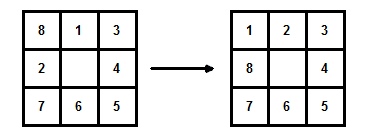
\includegraphics[scale=0.7]{chapters/informed_search/startziel.png}

Zur Anwendung von A* brauchen wir nun zunächst eine Heuristik, um die Anzahl der benötigten Züge zu schätzen. Eine mögliche Heuristik ist durch die Hamming-Distanz gegeben. Diese entspricht für einen gegebenen Zustand der Anzahl der Plättchen, welche an einer falschen Position (also nicht an ihrer Zielposition) liegen. Im Startzustand der obigen Abbildung beträgt diese Drei, da Kacheln 1, 2 und 8 verkehrt liegen.

\begin{description}
	\item[$h_{1}(n)$]{Anzahl falsch positionierter Kacheln in der durch Knoten $n$ dargestellten Konfiguration}
\end{description}

Eine weitere Bewertungsfunktion liefert die Manhattan-Distanz. In diesem Fall wird zu jeder Kachel zusätzlich geprüft, wie weit sie von ihrer korrekten Position entfernt liegt. Es wird also gezählt, wie oft die jeweilige Kachel verschoben werden müsste, um an ihrem korrekten Platz anzukommen, wenn keine anderen Kacheln im Weg lägen. Die entsprechende Heuristik ergibt sich dann als Summe der Distanzen der falsch positionierten Kacheln im Vergleich zur Zielkonfiguration. Im obigen Startzustand ergibt sich eine Manhattan-Distanz von Vier (Zwei für Kachel 2 und je Eins für Kacheln 1 und 8).

\begin{description}
	\item[$h_{2}(n)$]{Summe der Distanzen der falsch positionierten Kacheln zu ihrer Zielposition}
\end{description}

Wie man auf solche Bewertungsfunktionen kommt, werden wir im nächsten Unterkapitel behandeln. Sehen wir uns nun zunächst den konkreten Suchbaum  $G_{S1}$ an, welcher entsteht, wenn A* unter Verwendung von $h_{1}(n)$ auf das obige Problem angewendet wird.
Dieser ist in Abbildung \ref{fig:figure1} am Ende dieses Kapitels zu finden.

\begin{figure}[p]
	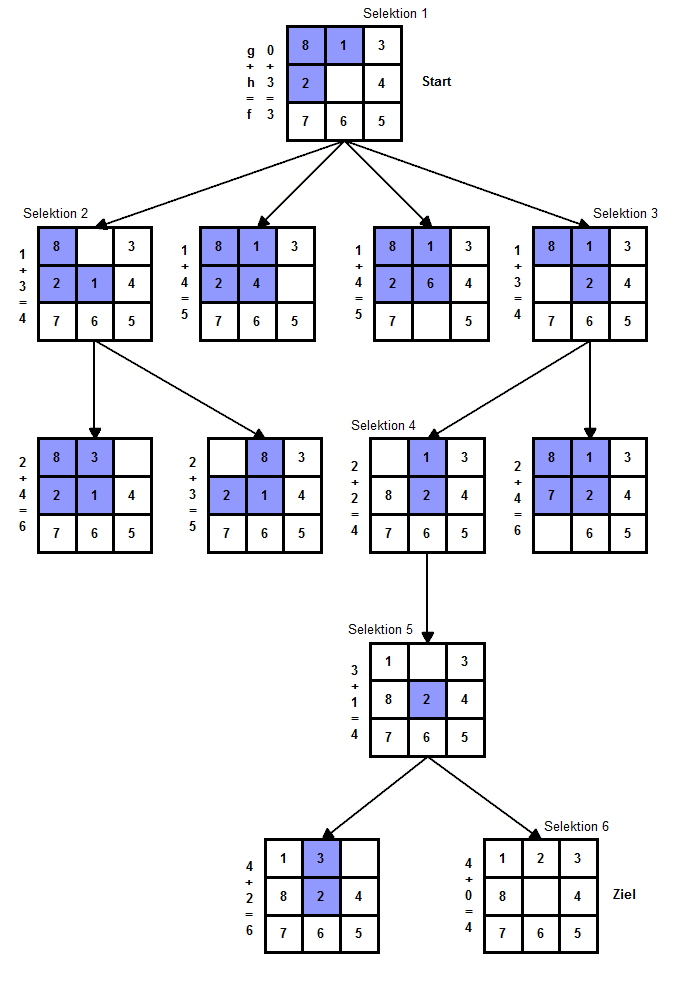
\includegraphics[width=14cm]{chapters/informed_search/tree1.png}
	\caption{Suchbaum $G_{S1}$ zu $h_{1}$}
	\label{fig:figure1}
\end{figure}

Die in der jeweiligen Konfiguration falsch liegenden Kacheln sind blau markiert. Die Werte $g(n)$, $h(n)$ und $f(n)$ sind jeweils linkerhand des Knotens $n$ angegeben. Weiterhin ist die Reihenfolge angegeben, in welcher die Knoten selektiert werden.
Der Such-Baum beginnt mit der Startkonfiguration in der Wurzel des Baumes und generiert daraufhin alle vier möglichen Nachfolger. Zu diesen werden mittels $g$ und der Heuristik $h_{1}$ die jeweiligen $f$-Werte berechnet. Von diesen wird nun der geringste Wert selektiert. Da von den vier Nachfolgern zwei den selben minimalen Wert besitzen, wird zufällig einer der beiden gewählt, in unserem Fall der Knoten ganz links. Dieser wird nun expandiert, indem wiederum seine möglichen Nachfolger generiert werden. Knoten, die zu Schleifen führen (also nur eine Operation rückgängig machen), lassen wir hier bewusst weg. Auch zu den neu generierten Knoten werden die $f$-Werte berechnet. Nun wird wiederum aus den noch nicht expandierten Knoten derjenige mit geringstem $f$-Wert selektiert. Dies trifft auf den Knoten rechts mit $f$-Wert 4 zu. Dieser wird nun expandiert. Nach weiteren Iterationen kommt es dann dazu, dass eine Zielkonfiguration generiert wird. Der zugehörige Knoten wird kurz darauf aufgrund seines minimalen $f$-Wertes selektiert und die Suche endet erfolgreich.

Für Heuristik $h_{2}(n)$ ergibt sich der folgende Suchbaum $G_{S2}$, welcher in Abbildung \ref{fig:figure2} am Ende dieses Kapitels zu finden ist.

\begin{figure}[p]
	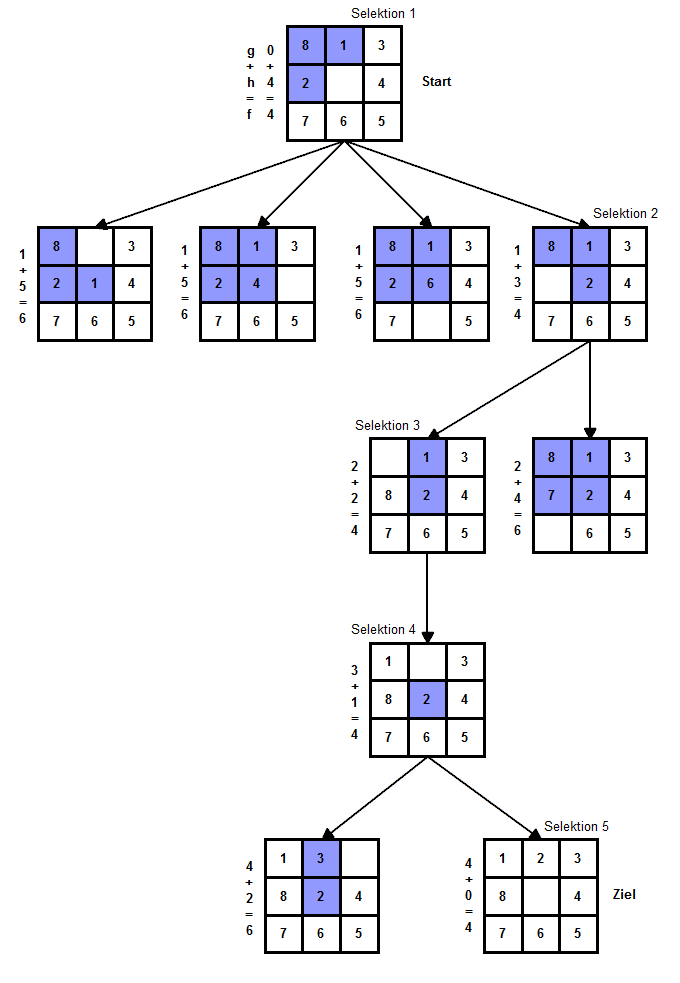
\includegraphics[width=14cm]{chapters/informed_search/tree2.png}
	\caption{Suchbaum $G_{S2}$ zu $h_{2}$}
	\label{fig:figure2}
\end{figure}

Wie wir sehen, ist hier eine geringere Anzahl von Expansionen nötig als bei unserer ersten Heuristik. Der Aufwand ist also geringer. Die Wahl des zu expandierenden Knotens ist stets eindeutig. Heuristik $h_{2}$ scheint also ein besserer Schätzer zu sein als $h_{1}$. Um zu verstehen, was einen vermeintlich guten Schätzer ausmacht, werden wir uns in Abschnitt \ref{theo} mit ein wenig Theorie beschäftigen und einige wünschenswerte Eigenschaften bezüglich Heuristikfunktionen und Suchverfahren kennenlernen.

%Zunächst möchte ich im folgenden jedoch eine konkrete Implementierung von A* festhalten.

%\subsection{Implementierung von A*}



%\glqq blinden\grqq

%\begin{SCfigure}
%	\centering
%	\includegraphics[width=0.8\textwidth]%
%	{tree1}% picture filename
%	\caption{Such-Baum zu h1}
%\end{SCfigure}


\section{Findung von Bewertungsfunktionen}

Im Beispiel des 8-Puzzles hatten wir folgende Vorbedingungen, welche erfüllt sein mussten, damit eine Verschiebe-Operation einer Kachel k von Feld x nach y ausgeführt werden konnte:
\begin{enumerate}
	\item Die Kachel k, welche bewegt werden soll, befindet sich auf Feld x.
	\item Feld y, in welches verschoben werden soll, ist benachbart zu Feld x.
	\item Dieses benachbarte Feld y ist leer -- dort befindet sich also keine Kachel.
\end{enumerate}
Die beiden im obigen Beispiel angegebenen Heuristiken $h_{1}(n)$ (Hamming-Distanz) und $h_{2}(n)$ (Manhattan-Distanz) sind durch Betrachten eines vereinfachten Modelles entstanden, bei welchem eine bzw. mehrere dieser konjunktiv verknüpften Bedingungen weggelassen wurden.
Betrachtet man das stark vereinfachte Modell, bei welchem zum Verschieben einer Kachel nur Bedingung 1 erfüllt sein muss, so gelangen wir zu Heuristik $h_{1}(n)$, bei welcher jede falsch positionierte Kachel direkt an ihre Zielposition gebracht werden kann und somit genau eine Verschiebe-Operation benötigt.
Erweitert man dieses einfache Modell ein wenig, indem ebenfalls Bedingung 2 vorausgesetzt wird, so ergibt sich als Heuristik die Manhattan-Distanz $h_{2}(n)$.

Dieses Prinzip des Konstruierens von vereinfachten Modellen durch systematisches Weglassen konjunktiv verknüpfter Einschränkungen scheint auch allgemein eine gute Herangehensweise zu sein, um leicht heuristische Schätzungen zu ermitteln.
So erhalten wir mit dieser Technik auch in folgendem Beispiel eine einfache Heuristik.

\theoremstyle{definition}
\newtheorem*{bsp}{Beispiel}
\begin{bsp}
	Gegeben ist ein Karte mit einem Straßennetz, sowie ein Start- und ein Endpunkt auf dieser Karte. Gesucht ist nun die kürzeste Verbindung vom Start zum Ziel, wobei nur die Wege dieser Karte verwendet werden dürfen. Lässt man die letztere Bedingung außer Acht, so erhält man eine für dieses Problem geeignete Heuristik: die Luftlinie zwischen dem betrachteten Knoten und dem Zielknoten.
\end{bsp}

\section{Theorie} \label{theo}

\theoremstyle{plain} %oder definition
\newtheorem*{zul}{Zulässigkeit}
\newtheorem*{os}{optimistische Schätzung}
\newtheorem*{zula}{Zulässigkeit von A*}

\subsection{Zulässigkeit eines Such-Verfahrens (insbesondere A*)}

Welche Bedingungen muss eine Heuristik erfüllen, damit unser Such-Verfahren ordnungsgemäß funktioniert? Dazu sollten wir zuerst definieren, wie wir uns ein korrekte Funktionsweise vorstellen.

\begin{zul}
	Ein Such-Verfahren heißt zulässig, falls es stets mit einer optimalen Lösung terminiert, falls diese existiert.
\end{zul}

Da bei unserem heuristischen Such-Verfahren A* die Wahl der Heuristik bisher nicht klar eingeschränkt ist, liegt es nahe, dass in dieser Wahl ein entscheidender Punkt für die Zulässigkeit unseres Algorithmus liegt. Man kann sich leicht Heuristiken überlegen, welche die Funktionsweise von A* stören und dafür sorgen, dass der Algorithmus keine optimale Lösung findet oder womöglich gar nicht erst terminiert.

Wir sollten uns also genauer mit der Beschaffenheit von Heuristikfunktionen auseinandersetzen.
Eine erste wichtige Eigenschaft einer Heuristik $h$ zur Schätzung von $h^{*}$ ist, ob diese optimistisch schätzt.

\begin{os}
Eine Schätzung $h$ von $h^{*}$ ist genau dann eine optimistische Schätzung, falls sie die Kosten eines optimalen Pfades nie überschätzt. Das heißt:
\[h(n) \leq h^{*}(n) \textrm{ für alle Knoten } n \in G_{P}\]
\end{os}

Die von uns aufgestellten Heuristiken $h_{1}$ und $h_{2}$ zur Schätzung der Züge im 8-Puzzle erfüllen dieses Kriterium und sind beide optimistische Schätzungen.
Diese Eigenschaft liefert uns nun die ausschlaggebende Bedingung für die Zulässigkeit von A*.

\begin{zula}
Falls die verwendete Heuristik $h$ eine optimistische Schätzung von $h^{*}$ ist, dann ist A* zulässig.
\end{zula}

Der Beweis dieses Satzes und einige genauere Erörterungen können in \cite{kaindl} nachgelesen werden.

\subsection{Eigenschaften von Heuristiken}

In diesem Kapitel sollen einige interessante Eigenschaften bezüglich Heuristikfunktionen erörtert werden.
Die Definitionen wurden aus \cite{kaindl} übernommen.
\theoremstyle{plain} %oder definition
\newtheorem*{theor}{Theorem}
\theoremstyle{definition}
\newtheorem*{defi}{Definition}

\begin{theor}
		$A_{1}^{*}$ und $A_{2}^{*}$ seien zwei Versionen von $A^{*}$ mit $h_{1}(n) \leq h^{*}(n)$ und $h_{2}(n) \leq h^{*}(n)$ für alle Knoten $n \in G$ und mit $h_{1}(n) \leq h_{2}(n)$ für alle Knoten $n \in G$ \textbackslash \ $\{$t $|$ t erfüllt die Endbedingung $\}$. ($A_{2}^{*}$ sei \glqq besser informiert\grqq\ als $A_{1}^{*}$.) Falls es eine Lösung gibt, so wird bis zur Terminierung jeder von $A_{2}^{*}$ expandierte Knoten auch von $A_{1}^{*}$ expandiert, ($A_{2}^{*}$ \glqq dominiert\grqq\ $A_{1}^{*}$.)
\end{theor}

\begin{defi}
	Eine heuristische Funktion $h(n)$ ist konsistent, wenn für alle Knotenpaare $m,n \in G$ folgendes erfüllt ist: \[h(m)\leq k(m,n)+h(n)\] mit $k(m,n)$ also Kosten des \glqq billigsten\grqq\ Pfades von $m$ nach $n$ ($k(m,n) = \infty$, wenn $n$ von $m$ aus nicht erreichbar ist); und für alle Knoten $t \in G$, die die Endbedingung erfüllen, gilt: \[h(t)=0\textrm{.}\]
\end{defi}

\begin{defi}
	Eine heuristische Funktion $h(n)$ ist monoton, wenn für alle Knotenpaare $m,n \in G$ mit $n$ als unmittelbarem Nachbar von $m$ folgendes erfüllt ist: \[h(m)\leq c(m,n)+h(n)\] mit $c(m,n)$ als Kosten der Kante von $m$ nach $n$; und für alle Knoten $t \in G$, die die Endbedingung erfüllen, gilt: \[h(t)=0\textrm{.}\]
\end{defi}

\begin{theor}
	Die Eigenschaften konsistent und monoton sind äquivalent.
\end{theor}

\begin{theor}
	Für jede konsistente Funktion h gilt: \[h(n)\leq h^{*}(n)\textrm{ für alle Knoten } n \in G\]
\end{theor}
Jede konsistente bzw. monotone Funktion $h$ schätzt also optimistisch. Dadurch ist $A^{*}$ unter Verwendung von konsistentem h zulässig.

\subsection{Komplexität von A*}

Es lässt sich leicht erkennen, dass A* in der Regel eine weit bessere Komplexität hat, als blinde Such-Verfahren. Die Anzahl der expandierten Knoten ist bei A* oft sogar um ein Vielfaches geringer. Sei nun die Länge einer optimalen Lösung mit $d$ bezeichnet. Des Weiteren kann man von Einheitskosten ausgehen und die Existenz genau einer optimalen Lösung voraussetzen.
Je nachdem wie optimistisch nun der Fehler von $h$ bezüglich $h^{*}$ angenommen wird, kommt man auf eine quadratische oder sogar lineare Komplexität bezüglich d. Im eher realistischen Fall lässt sich jedoch nur auf eine exponentielle Komplexität schließen.
\subsection{Optimalität von A*}

Nun interessieren wir uns für die Optimalität von A* im Hinblick auf die Anzahl der expandierten Knoten.
Der Begriff Optimalität beruht hier auf dem der Dominanz. Das bedeutet, ein Verfahren ist optimal gegenüber einer Klasse von Verfahren, wenn es alle Elemente aus dieser Klasse dominiert.

Für den ganz allgemeinen Fall lässt sich leicht erkennen, dass A* nicht \textit{das} optimale Verfahren überhaupt ist. Es gibt in bestimmten Fällen offensichtlich Verfahren, welche nicht alle von A* untersuchten Knoten ebenfalls untersuchen. Gerade bei speziell auf eine Klasse von Graphen abgestimmten Verfahren ist dies der Fall.

Jedoch ist unter bestimmten Einschränkungen eine konkretere Aussage bezüglich der Optimalität von A* möglich. Dafür schränkt man die Bedingungen auf eine Domäne ein, welche eine konsistente Heuristik $h$ besitzt, und setzt voraus, dass es mindestens einen optimalen Lösungspfad gibt, bei welchem $h < h^{*}$ für alle Knoten außer dem Zielknoten gilt. Dann gilt, dass A* dominant für alle Problem-Instanzen ist, und zwar für alle möglichen Entscheidungsregeln bei Nicht-Eindeutigkeit des Knotens mit minimalem $f$-Wert. Da dem Algorithmus A* bei konsistentem h zusätzlich eine sehr gute Verwaltung des Suchbaumes möglich ist, lässt sich sagen, dass A* unter diesen Voraussetzungen sehr effektiv ist.
